\documentclass[a4paper,12pt]{article}
\usepackage[utf8]{inputenc}
\usepackage[T1]{fontenc}
\usepackage{lmodern}
\usepackage{booktabs}
\usepackage{graphicx}
\usepackage{caption}
\usepackage{geometry}
\geometry{margin=1in}

\title{Appendix}
\date{}             % đặt ngày rỗng
\renewcommand{\date}[0]{}   % chắc chắn ghi đè mọi định nghĩa cũ

\begin{document}
\maketitle

\appendix

%---------------------------------------------
\section{Hanami Language Reference}
\label{appendix:language-reference}

\subsection{Keyword Mapping}
\begin{table}[h!]
  \centering
  \caption{Core Hanami keywords and their C++ equivalents}
  \begin{tabular}{llp{6cm}}
    \toprule
    \textbf{Hanami} & \textbf{C++ Equivalent} & \textbf{Meaning} \\
    \midrule
    \texttt{garden <Name>}        & \texttt{namespace <Name>{...}}    & Declares a namespace \\
    \texttt{species <Name>}       & \texttt{class <Name>{...}}        & Declares a class \\
    \texttt{open:}                & \texttt{public:}                  & Public section specifier \\
    \texttt{hidden:}              & \texttt{private:}                 & Private section specifier \\
    \texttt{grow <f>(...) -> <t>} & \texttt{<t> <f>(...)}             & Declares a function \\
    \texttt{bloom << x;}          & \texttt{std::cout << x;}         & Console output \\
    \texttt{water >> x;}          & \texttt{std::cin >> x;}          & Console input \\
    \texttt{branch (cond){...}}   & \texttt{if (cond){...}}           & If statement \\
    \texttt{else branch (cond)}   & \texttt{else if (cond)}           & Else-if clause \\
    \texttt{else {...}}           & \texttt{else {...}}               & Else clause \\
    \bottomrule
  \end{tabular}
\end{table}

%---------------------------------------------
\section{UML Diagrams}
\noindent
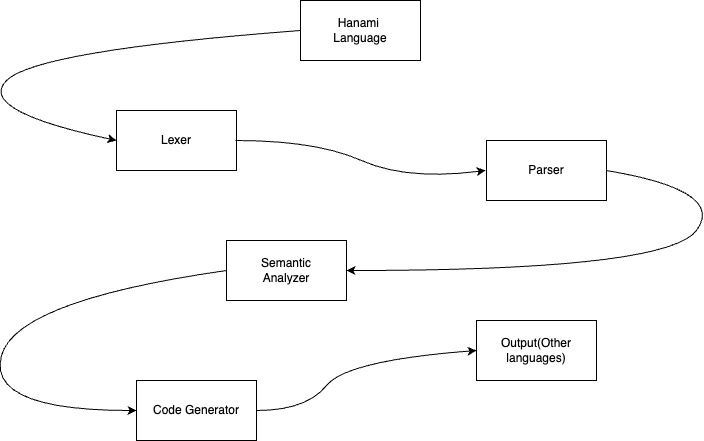
\includegraphics[
 width=1.1\textwidth,
 height=0.80\textheight,
]{UMLDiagram (1).jpg}
\captionof{figure}{High-level flow from Hanami Language through Lexer, Parser, Semantic Analyzer, to Code Generator and target outputs.}\medskip

\section{Semantic Analyzer Visitor}
\noindent
\label{appendix:codegen}

% Mũi tên chỉ quan hệ kế thừa (“extends”)

% Page 1
\noindent
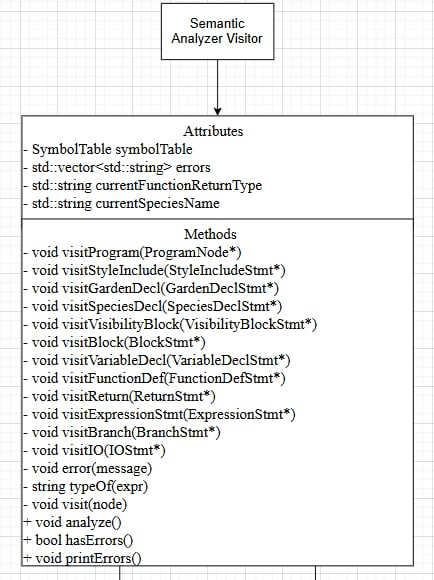
\includegraphics[
  width=0.95\textwidth,    % 95% chiều rộng trang
  height=0.95\textheight,                 % 95% chiều cao trang
  keepaspectratio                         % giữ tỉ lệ gốc
]{Semantic_Analyzer1 (1).jpg}
\newpage
% Page 2
\noindent
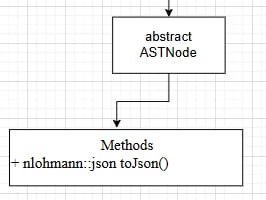
\includegraphics[
 width=0.95\textwidth,    % 95% chiều rộng trang
  height=0.90\textheight,                 % 95% chiều cao trang
  keepaspectratio                         % giữ tỉ lệ gốc
  ]{Semantic_Analyzer2 (1).jpg}
\newpage

% Page 3
\noindent
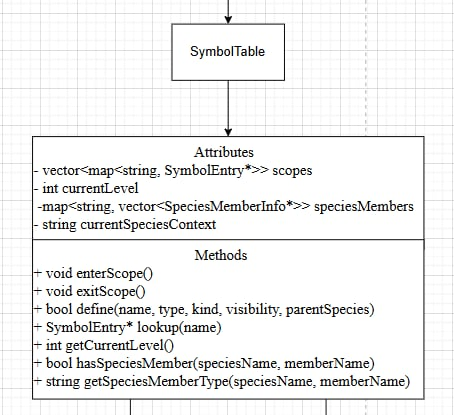
\includegraphics[
 width=0.95\textwidth,    % 95% chiều rộng trang
  height=0.90\textheight,                 % 95% chiều cao trang
  keepaspectratio                         % giữ tỉ lệ gốc
  ]{Semantic_Analyzer3 (1).jpg}
\newpage


% Page 4: Semantic Analyzer (cuối cùng) — thu nhỏ để chứa caption
\noindent
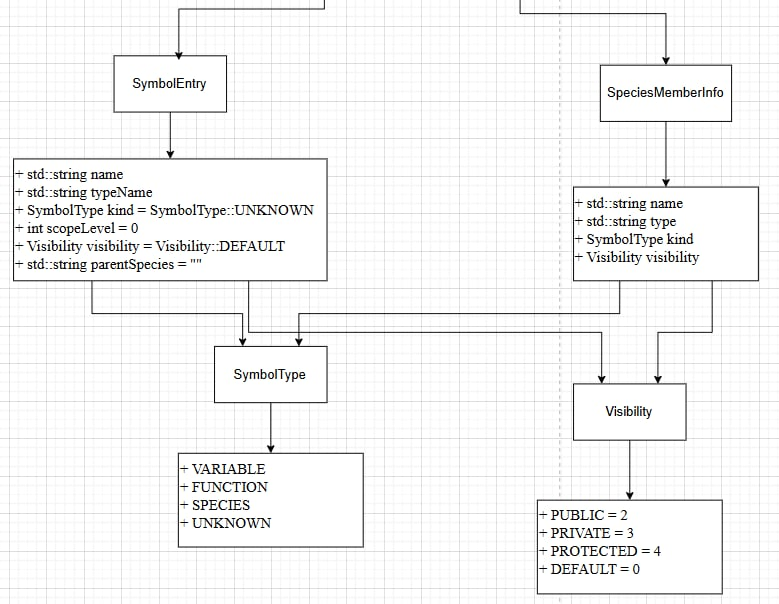
\includegraphics[
  width=\textwidth,
  height=0.80\textheight,    % giảm so với 0.96 lên 0.88
]{Semantic_Analyzer4 (1).jpg}
               % chút khoảng cách cho caption
\captionof{figure}{Class diagram of the Semantic Analyzer visitor, symbol table, and related entries.}
\label{fig:semantic-analyzer-full}

\newpage


%---------------------------------------------
\section{Parser Structure (Part 1)}
\noindent
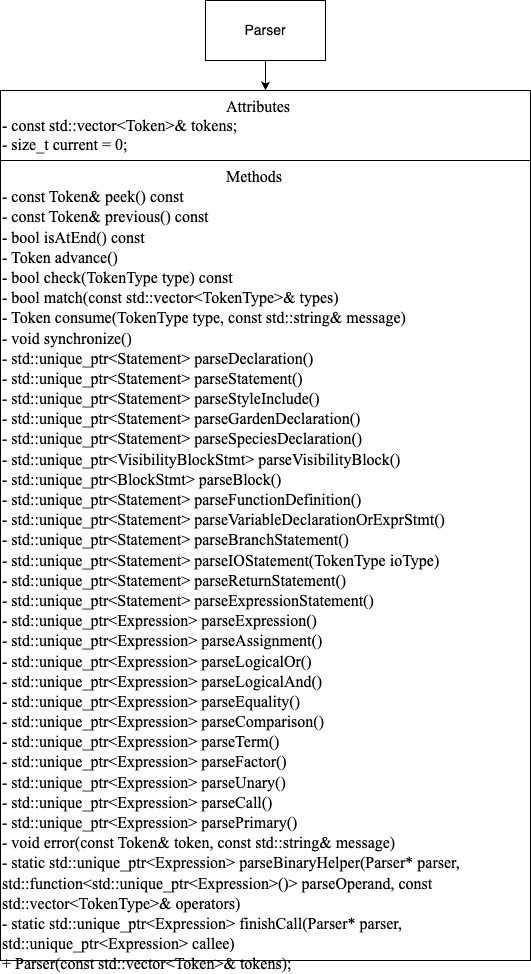
\includegraphics[
  width=0.9\textwidth,
  height=0.7\textheight,
  trim=0 500 0 0,clip]{Parser (1).jpg}
\captionof{figure}{Parser class attributes and parsing methods (overview, part 1).}\medskip

\section{Parser Structure (Part 2)}
\noindent
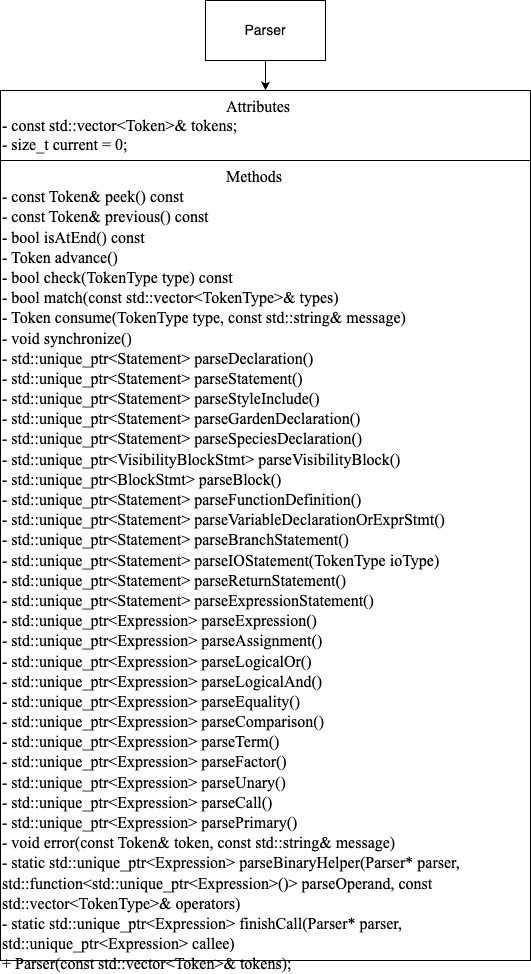
\includegraphics[
  width=0.9\textwidth,
  height=0.7\textheight,
  trim=0 0 0 500,clip]{Parser (1).jpg}
\captionof{figure}{Parser class attributes and parsing methods (details, part 2).}\medskip

%---------------------------------------------
\section{Lexer Implementation}
\label{appendix:lexer}

% Part 1: Top of class (attributes)
\noindent
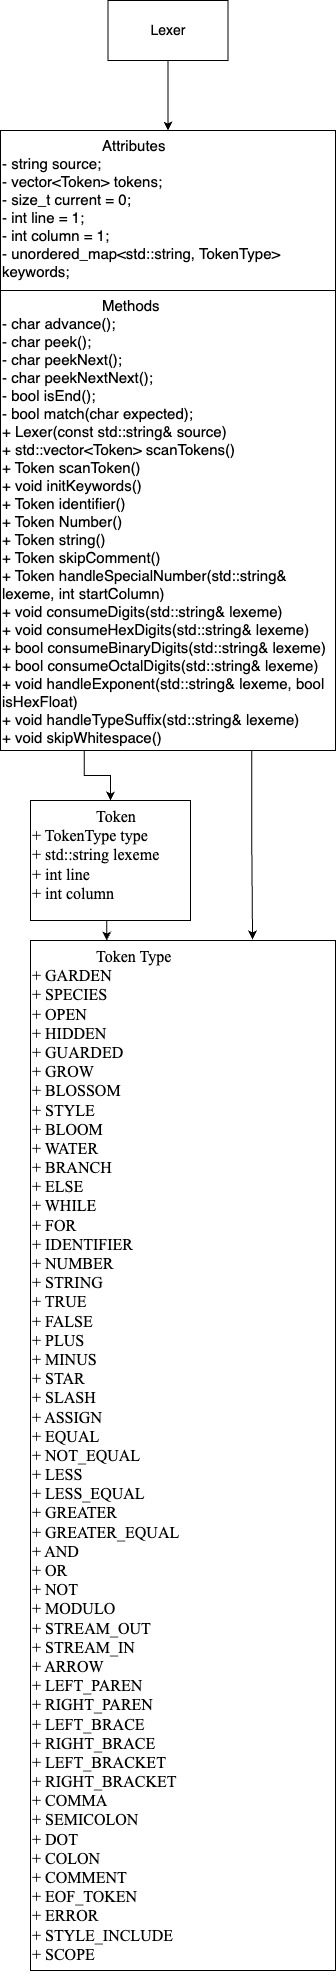
\includegraphics[
  width=0.90\textwidth,
  height=0.75\textheight,
  keepaspectratio,
  trim=0 1600 0 0,clip
]{Lexer (1).jpg}

\newpage
% Part 2: Upper-middle (core scan methods)
\noindent
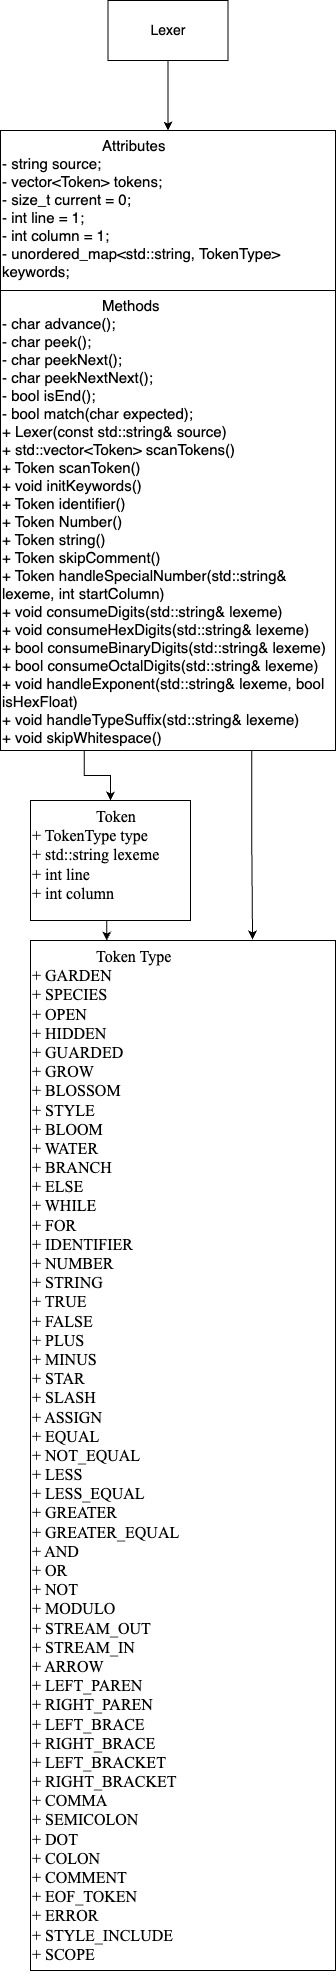
\includegraphics[
  width=0.90\textwidth,
  height=0.75\textheight,
  keepaspectratio,
  trim=0 1300 0 300,clip
]{Lexer (1).jpg}

\newpage
% Part 3: Middle (helper methods + start of Token struct)
\noindent
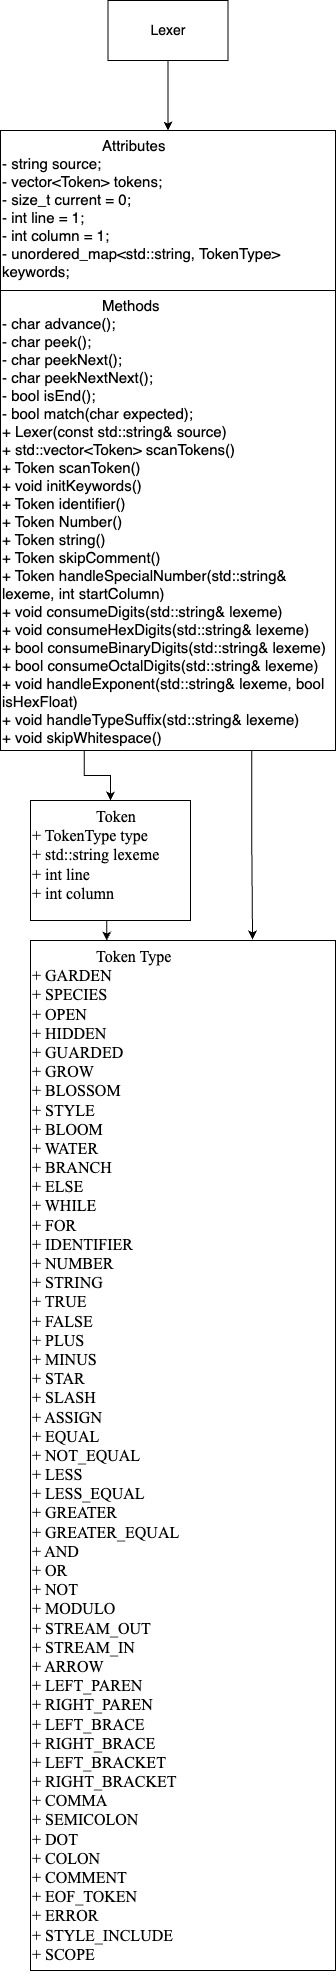
\includegraphics[
  width=0.90\textwidth,
  height=0.75\textheight,
  keepaspectratio,
  trim=0 1000 0 600,clip
]{Lexer (1).jpg}

\newpage
% Part 4: Lower-middle (Token struct + first half of TokenType)
\noindent
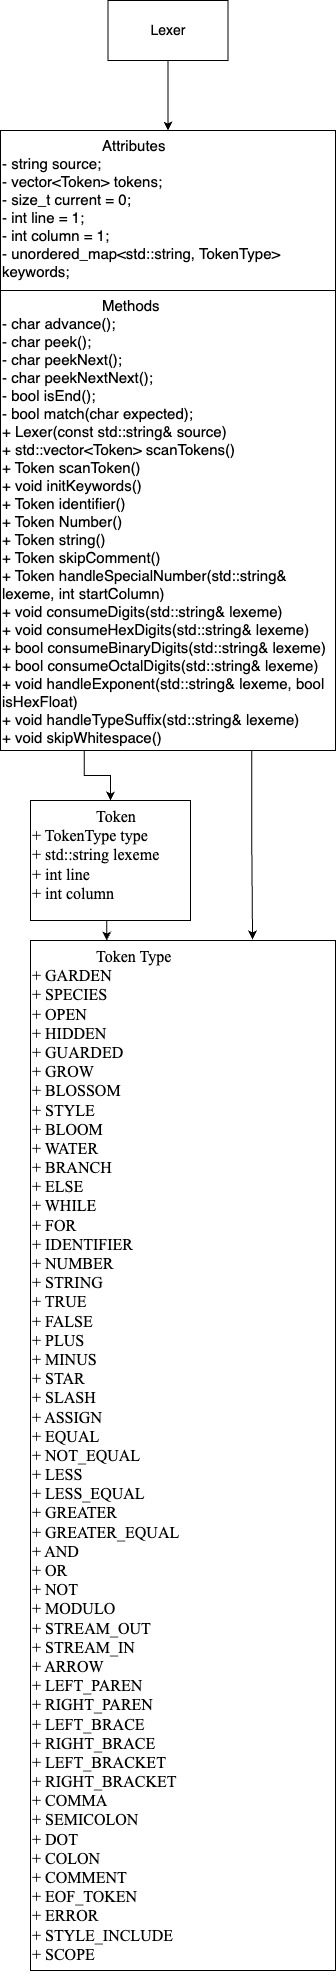
\includegraphics[
  width=0.90\textwidth,
  height=0.75\textheight,
  keepaspectratio,
  trim=0 700 0 900,clip
]{Lexer (1).jpg}

\newpage
% Part 5: Upper TokenType entries (TRUE … LEFT_BRACKET)
\noindent
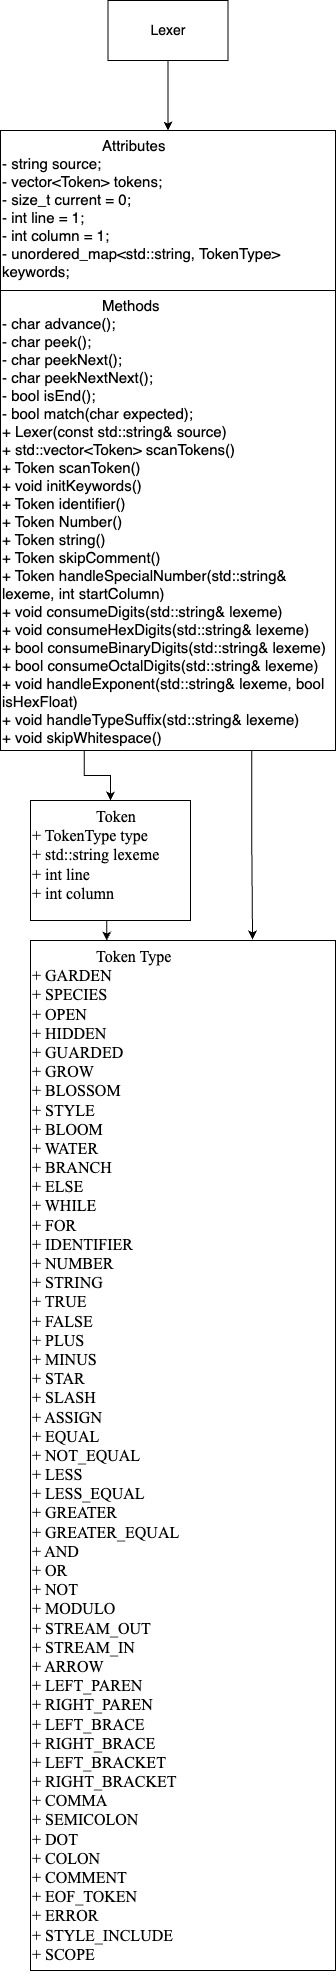
\includegraphics[
  width=0.90\textwidth,
  height=0.75\textheight,
  keepaspectratio,
  trim=0 400 0 1200,clip
]{Lexer (1).jpg}

% (sau đó Part 6 và caption như bạn đã chỉnh)


\newpage
% Part 6: Remaining TokenType entries (RIGHT_BRACE … SCOPE)
\noindent
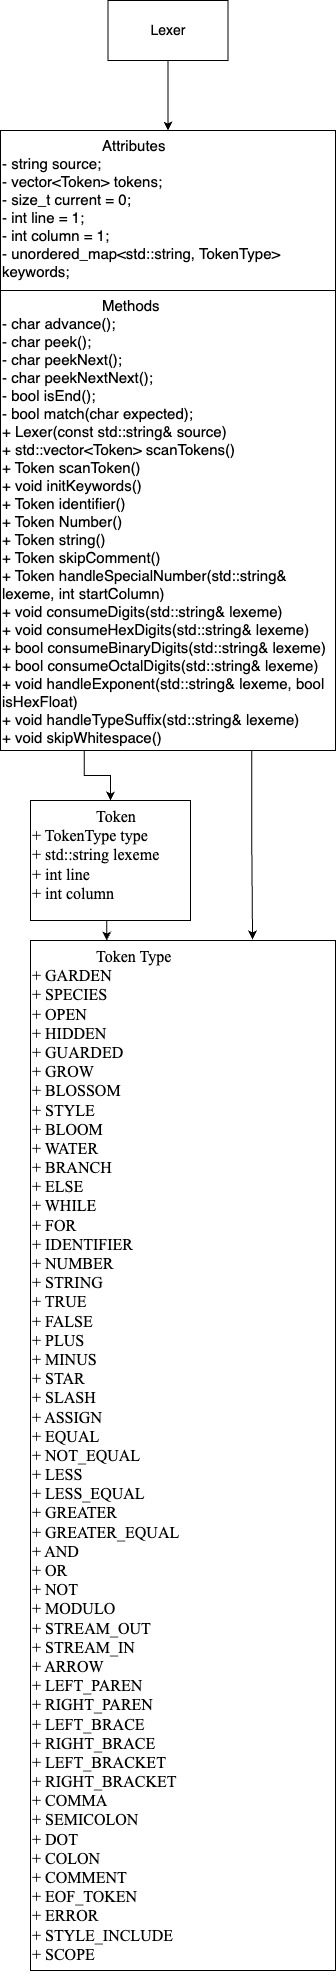
\includegraphics[
  width=0.95\textwidth,      % thu nhỏ xuống 90% chiều rộng trang
  height=0.90\textheight,    % thu nhỏ xuống 75% chiều cao trang
  keepaspectratio,           % giữ tỉ lệ gốc
  trim=0 0 0 1400,clip       % cắt đúng phần RIGHT_BRACE … SCOPE
]{Lexer (1).jpg}

\captionof{figure}{Complete \texttt{Lexer} class UML split across six pages to show all attributes, methods, the \texttt{Token} struct, and the entire \texttt{TokenType} enumeration (from \texttt{RIGHT\_BRACE} through \texttt{SCOPE}).}
\label{fig:lexer-full}

\newpage


%---------------------------------------------
%---------------------------------------------
\section{Code Generator Visitor}
\label{appendix:codegen}

% Mũi tên chỉ quan hệ kế thừa (“extends”)

% Page 1
\noindent
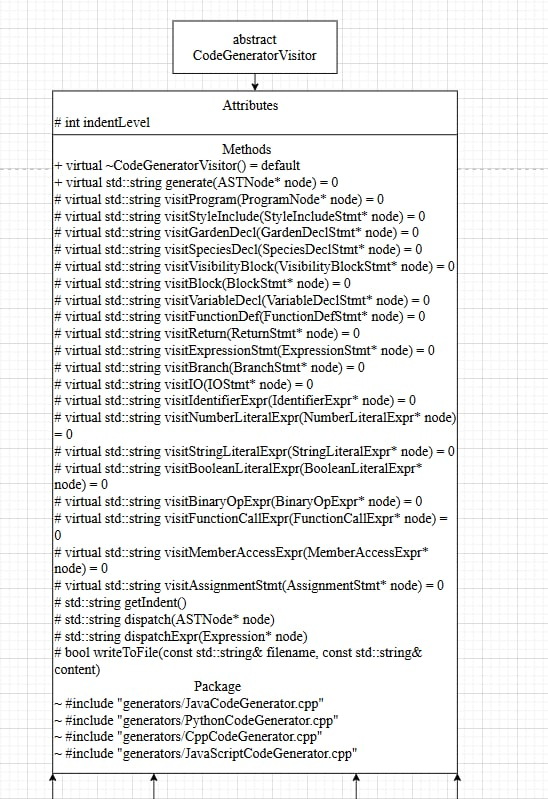
\includegraphics[
  width=0.95\textwidth,    % 95% chiều rộng trang
  height=0.95\textheight,                 % 95% chiều cao trang
  keepaspectratio                         % giữ tỉ lệ gốc
  ]{CodeGeneratorVisitor1 (1).jpg}
\newpage
% Page 2
\noindent
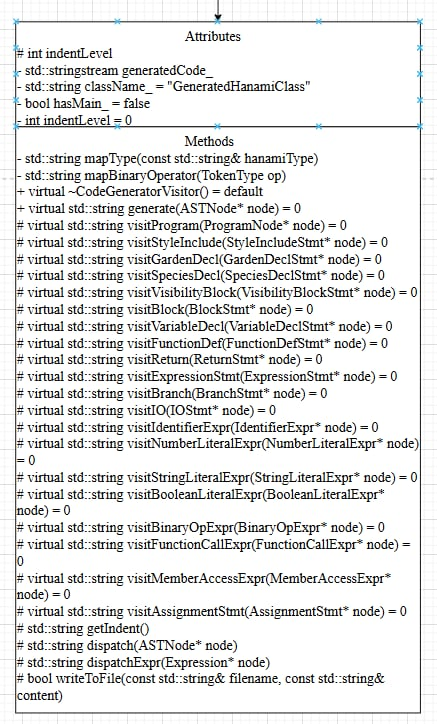
\includegraphics[
  width=0.95\textwidth,    % 95% chiều rộng trang
  height=0.95\textheight,                 % 95% chiều cao trang
  keepaspectratio                         % giữ tỉ lệ gốc
  ]{CodeGeneratorVisitor2 (1).jpg}
\newpage

% Page 3
\noindent
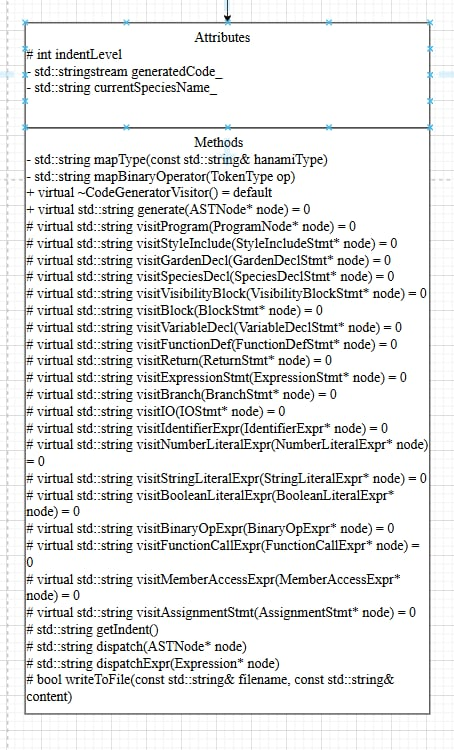
\includegraphics[
  width=0.95\textwidth,    % 95% chiều rộng trang
  height=0.95\textheight,                 % 95% chiều cao trang
  keepaspectratio                         % giữ tỉ lệ gốc
  ]{CodeGeneratorVisitor3 (1).jpg}
\newpage

% Page 4
\noindent
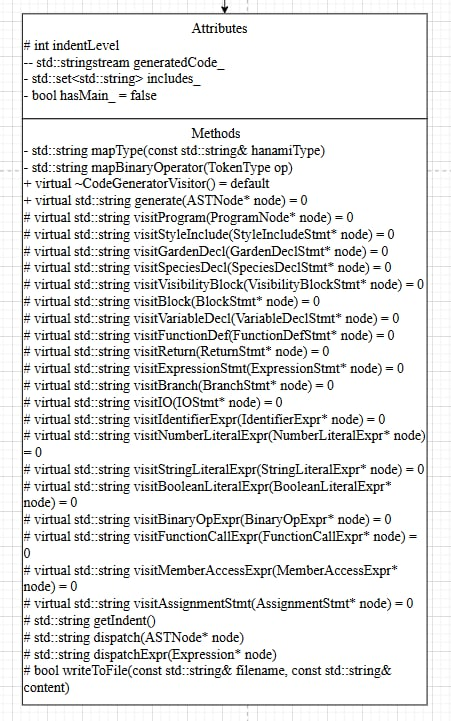
\includegraphics[
 width=0.95\textwidth,    % 95% chiều rộng trang
  height=0.95\textheight,                 % 95% chiều cao trang
  keepaspectratio                         % giữ tỉ lệ gốc
  ]{CodeGeneratorVisitor4 (1).jpg}
\newpage

% Page 5 + caption, ảnh bé hơn để nhét caption
\noindent
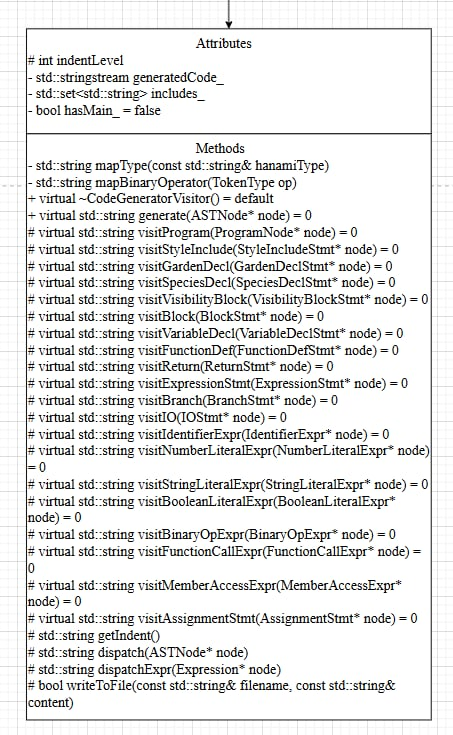
\includegraphics[
  width=0.95\textwidth,      % 95% chiều rộng trang
  height=0.95\textheight,    % 95% chiều cao trang
  keepaspectratio           % giữ tỉ lệ gốc
]{CodeGeneratorVisitor5 (1).jpg}

\captionof{figure}{Abstract \texttt{CodeGeneratorVisitor}.}
\label{fig:cgvisitor-full}

\newpage

%---------------------------------------------
\section{IR-Based Code Generator}

\noindent
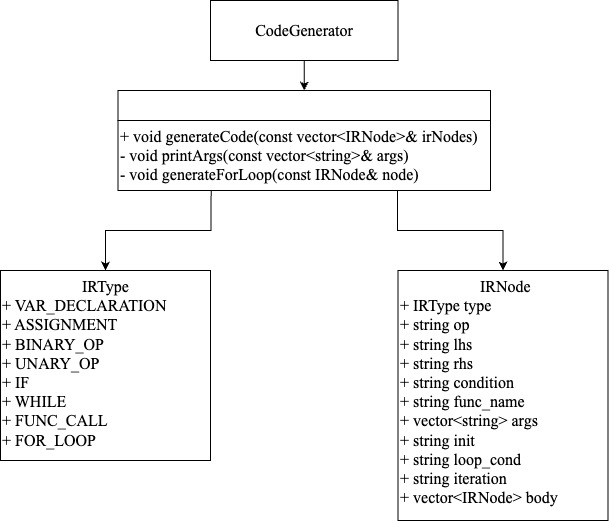
\includegraphics[
  width=0.99\textwidth,
  height=0.80\textheight, 
]{CodeGenerator (1).jpg}

\captionof{figure}{CodeGenerator class overview with IR types and generation routines.}\medskip
\label{appendix:ir}

%---------------------------------------------
\section{Sequence Diagram}
\label{appendix:sequence}

\noindent
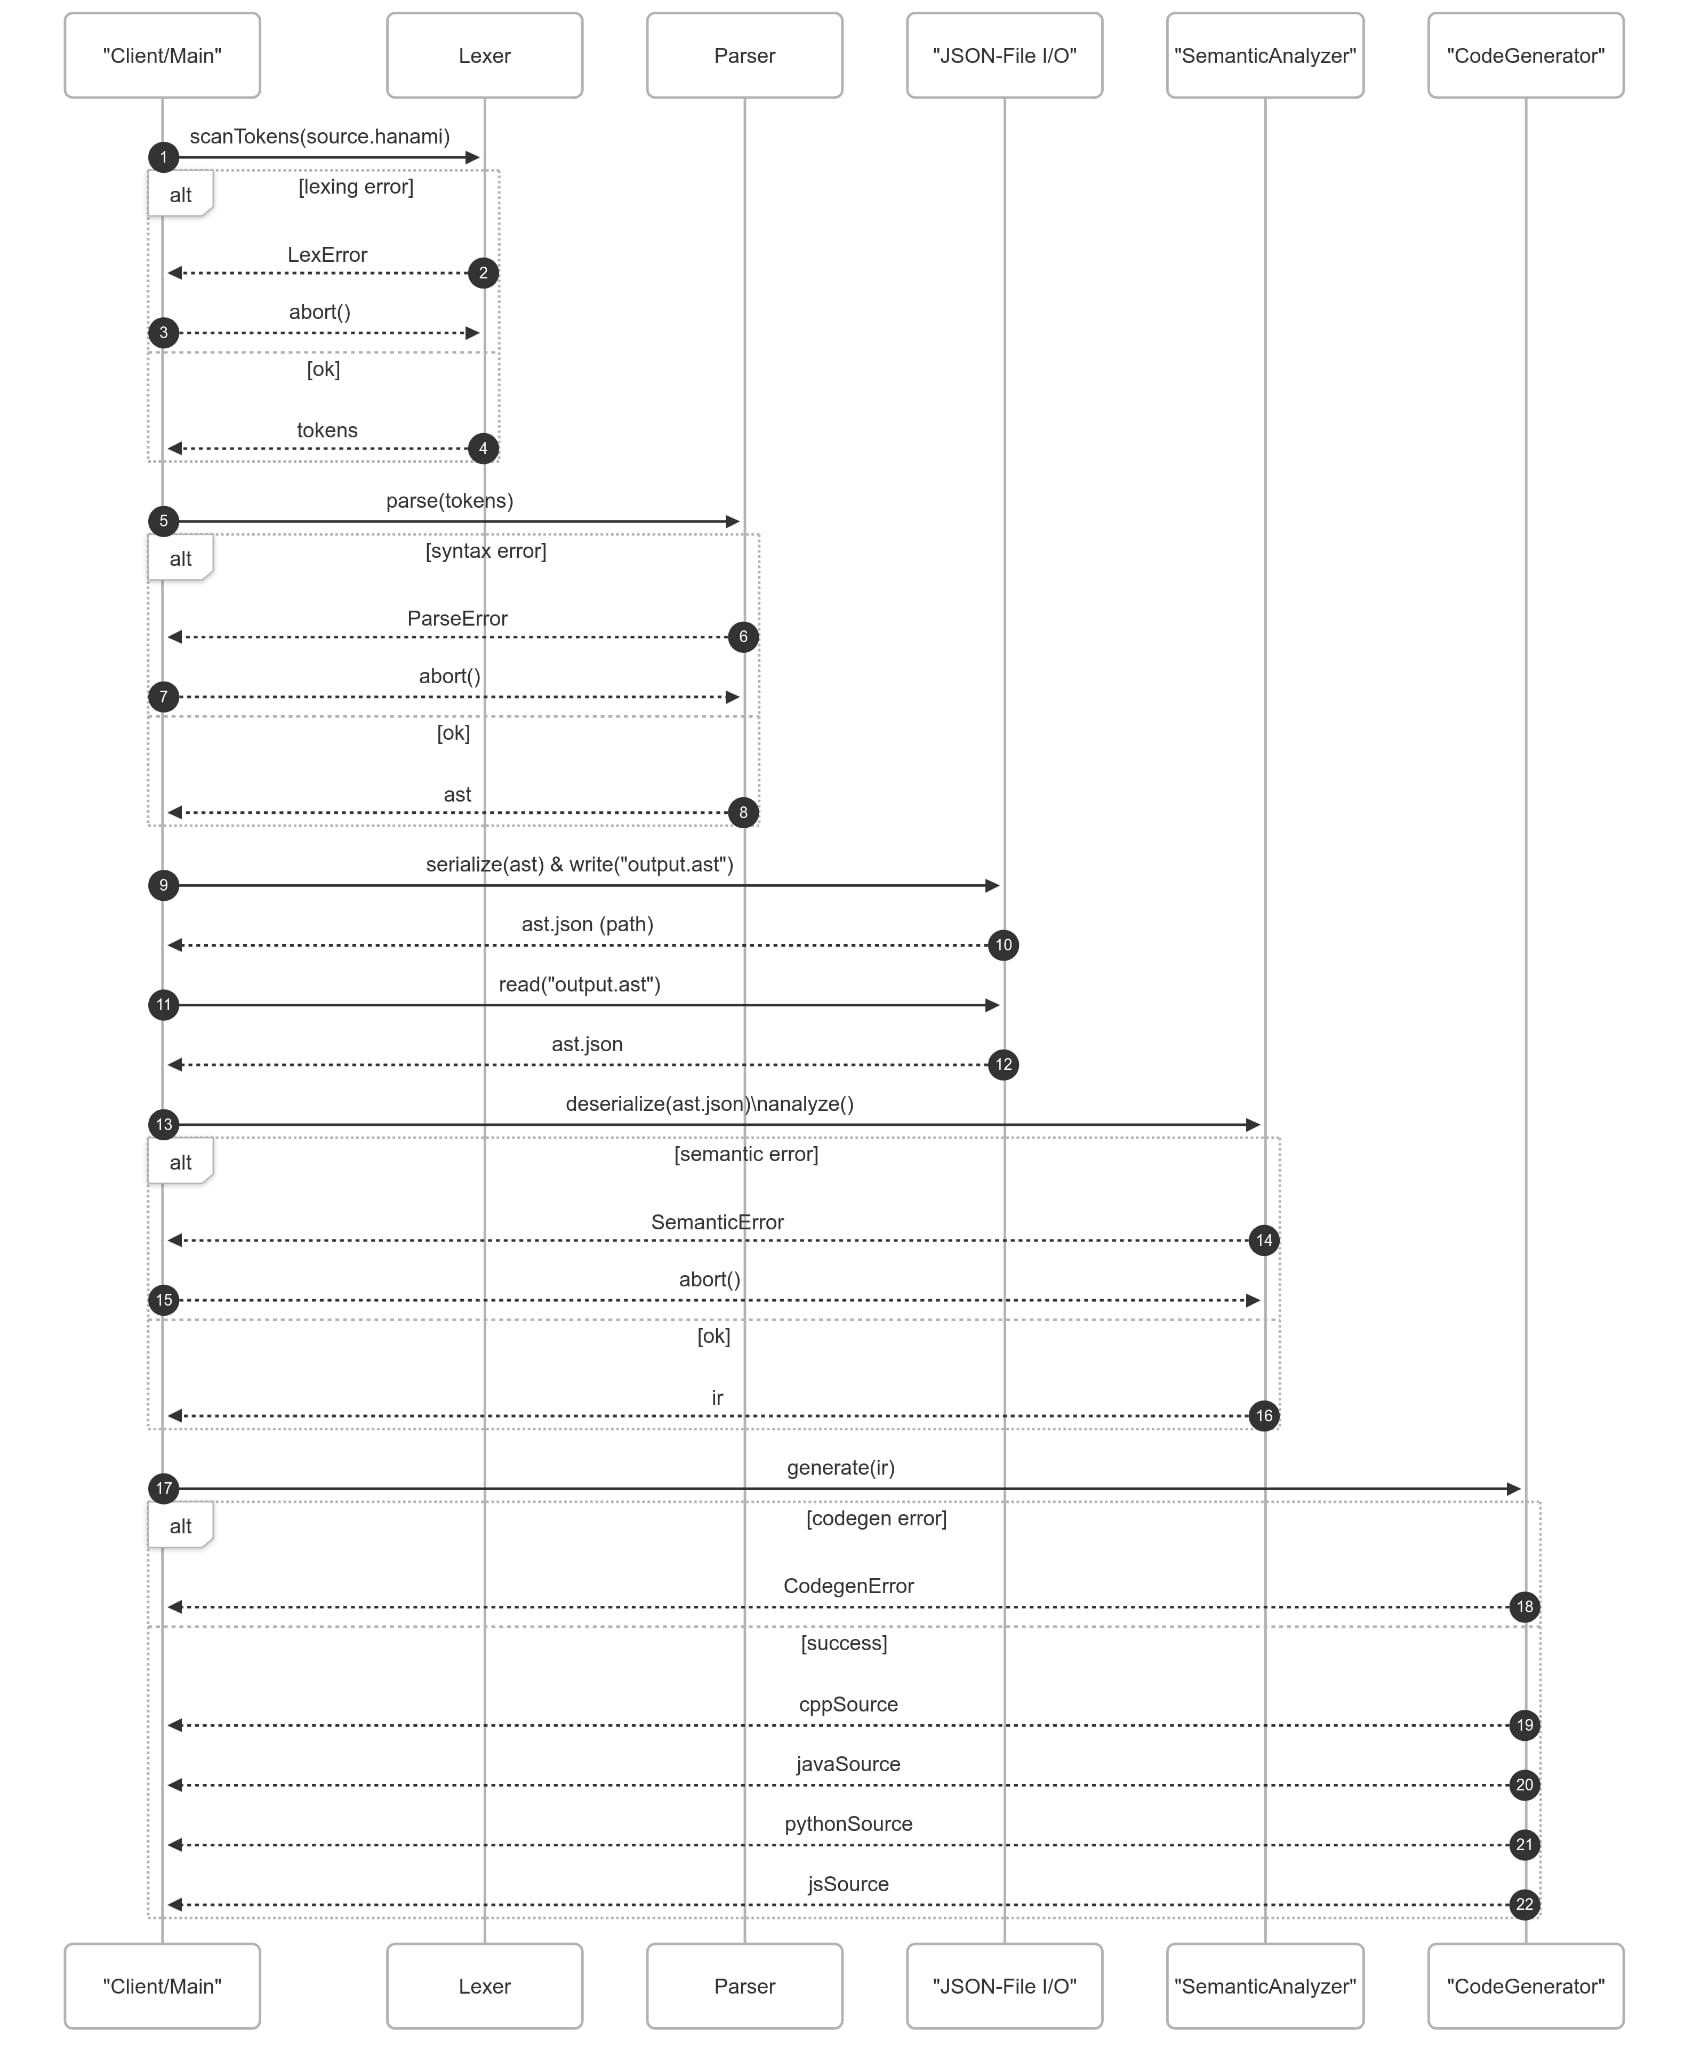
\includegraphics[width=\textwidth]{sequence.jpeg}
\captionof{figure}{End-to-end sequence diagram depicting interactions between Client/Main, Lexer, Parser, JSON I/O, Semantic Analyzer, and Code Generator.}

\end{document}
